%%%%%%%%%%%%%%%%%%%%%%%%%%%%%%%%%%%%%%%%%%%%%%
% To select a journal, use its code for the 
% journal= option in the \documentclass command.
% The journal codes for this template are:
% 
% Annals of Actuarial Science: aas
% British Journal of Political Science: jps
% Network Science: nws
% Political Analysis: pla
% Political Science Research and Methods: ram
% Evolutionary Human Sciences: ehs
% Natural Language Processing: nlp
%%%%%%%%%%%%%%%%%%%%%%%%%%%%%%%%%%%%%%%%%%%%%%
\newcommand{\mm}{MM-DGAT}

\documentclass[
  journal=noname,
  manuscript=draft,
  year=,
  volume=,
]{cup-journal}

\usepackage{amsmath}
\usepackage[nopatch]{microtype}
\usepackage{booktabs}

\title{MM-DGAT: Multi-Modal Dynamic Graph Attention Networks via disease dependency learning}

\author{Giovanni Officioso}
\affiliation{University of Milán-Bicocca, DEMS, Milán, Italy}
\email[Giovanni Officioso]{g.officioso@campus.unimib.it}

% \author{S. Author}
% \affiliation{Second Division, Organization, City, Pincode, State, Country}
% % \alsoaffiliation{Joint first authors}

% \author{T. Author}
% \affiliation{Second Division, Organization, City, Pincode, State, Country}

% \author{F.T. Author}
% \affiliation{Fourth Division, Organization, City, Pincode, State, Country}

\addbibresource{example.bib}

\keywords{Graph attention networks, Multi-label classification, Multi-modal classifikcation framework} %% First letter not capped

\begin{document}

\begin{abstract}

Accurate multi-label chest X-ray classification is essential for automated medical diagnosis, yet remains challenging due to complex inter-disease relationships that vary across patient presentations. 

Existing approaches face two fundamental limitations: they either treat disease labels independently, ignoring clinical co-occurrence patterns or employ static disease correlation graphs that cannot adapt to individual cases. Moreover, current methods operate solely on visual features, disregarding the rich contextual information available in radiology reports. 

We propose \textbf{\mm}\, (Multi-Modal Dynamic Graph Attention  Networks), the first approach to generate patient-specific, multi-modal-conditioned disease correlation graphs for chest X-ray  diagnosis. MM-DGAT addresses these limitations through three key innovations:
\begin{enumerate}
    \item cross-modal fusion that integrates visual features from radiographs with textual embeddings provided by clinical reports via attention mechanisms;
    \item dynamic graph generation that produces  adaptive disease correlation structures conditioned on fused  multi-modal representations; 
    \item graph attention networks that perform context-aware message passing over these patient- specific graphs. 
\end{enumerate}

% Multi-label chest X-ray classification traditionally relies on imaging features alone, ignoring the rich textual information in radiology reports. Moreover, existing graph-based methods use static disease correlation graphs that fail to adapt to individual patient presentations. Here is proposed \textbf{MM-DGAT} (Multi-Modal Dynamic Graph Attention Networks), the first approach to generate image and text-conditioned dynamic graphs for chest X-ray diagnosis. This model: 
% \begin{enumerate}
%     \item fuses visual and textual features via cross-attention;
%     \item generates patient-specific disease correlation graphs;
%     \item performs adaptive message passing.
% \end{enumerate} 
\end{abstract}

\section{Introduction}
\label{sec:introduction}

Medical image diagnosis represents one of the most critical yet  challenging applications of computer vision, where accurate  identification of multiple co-occurring pathologies directly impacts  patient care and clinical outcomes. Among medical imaging modalities, chest radiography (chest X-ray, CXR) stands as the most frequently performed diagnostic examination worldwide\autocite{techspec}, serving as the first-line tool for detecting thoracic diseases ranging from pneumonia and tuberculosis to cardiovascular conditions and malignancies. The interpretation of chest X-rays demands not only the recognition of individual pathologies but also understanding the complex clinical relationships between diseases that frequently co-occur in predictable patterns.

\subsection{Motivation and Clinical Context}

While deep learning has achieved remarkable success in single-label image classification\autocite{he2015deepresiduallearningimage}, multi-label medical diagnosis presents substantially greater challenges. Indeed this task requires simultaneous identification of multiple pathologies, each potentially presenting with varying severity and spatial distribution. More critically, diseases do not occur in isolation. For instance cardiomegaly frequently accompanies pulmonary edema due to shared cardiovascular pathophysiology, or pneumonia often presents alongside consolidation and infiltration or pleural effusion may indicate underlying malignancy, infection, or cardiac failure depending on the clinical context.

These disease co-occurrence patterns reflect fundamental aspects of human pathophysiology and represent crucial diagnostic knowledge that radiologists leverage during interpretation. However, the relationships between diseases are not uniform across all patients. Consider two patients presenting with pleural effusion: in the first case, it may co-occur with cardiomegaly in the context of congestive heart failure, exhibiting a strong positive correlation. In the second case, the same finding may appear alongside pneumonia in an infectious setting, demonstrating an entirely different correlation pattern. This \textit{patient-specific} nature of disease relationships poses the following question: how can we build models that capture both the general statistical tendencies of disease co-occurrence and the specific manifestations in individual cases?

Moreover, radiologists do not interpret images in isolation. Indeed clinical reports containing patient history, symptoms, and prior findings, provide essential context that influences image interpretation. A radiograph showing mild cardiomegaly may be interpreted differently when accompanied by a report stating phrases like \textit{"known history of congestive heart failure"} or \textit{"acute chest pain with no prior cardiac history."} This integration of visual and textual information represents standard clinical practice, yet most automated systems operate solely on imaging features.

\subsection{Limitations of Current Approaches}

Current approaches to multi-label chest X-ray classification fall into three main categories, each with distinct limitations:
\begin{enumerate}
    \item label-independent;
    \item static graph-based;
    \item multi-modal.
\end{enumerate}

Label-independent methods employ standard deep learning architectures with independent binary classifiers for each disease\autocite{rajpurkar2017chexnetradiologistlevelpneumoniadetection}. While achieving strong performance through sophisticated architectures and large-scale training, these methods fundamentally ignore disease co-occurrence patterns. Each pathology is predicted independently, precluding the model from leveraging the rich correlations between diseases that human experts routinely exploit.

On the other hand static graph-based methods address this limitation by explicitly modeling disease relationships through graph neural networks\autocite{bbcgn}. These approaches construct a disease correlation graph, typically from training set co-occurrence statistics, and use graph convolutional or attention mechanisms to propagate information between related diseases. While demonstrating clear improvements over independent classifiers, they employ \textit{fixed} graph structures: the same disease correlation matrix is applied to all patients, regardless of their specific presentation. This one-size-fits-all paradigm cannot capture the patient-specific variations in disease manifestations described above.

Last but not least, multi-modal methods leverage both imaging and textual information, primarily through vision-language models adapted to radiology\autocite{zhang2025biomedclipmultimodalbiomedicalfoundation}. These approaches typically focus on report generation or image-text retrieval tasks rather than structured classification. Crucially, they do not model disease relationships through explicit graph structures, treating diseases as independent despite their known clinical correlations.

Notably, no existing work combines all three capabilities: modeling disease relationships through graphs, adapting graph structure to individual patients and integrating multi-modal information. This represents a critical gap, as these three aspects are fundamentally complementary. Indeed disease relationships not only should be modeled (graphs), but also should adapt to specific cases (dynamics), and should be informed by all available information (multi-modality).

\subsection{Our Approach: MM-DGAT}

We propose \textbf{\mm} (Multi-Modal Dynamic Graph Attention 
Networks), a novel framework that addresses these limitations by 
introducing patient-specific multi-modal-conditioned disease 
correlation graphs, which is based on the key insight that disease relationship 
strengths should not be fixed, but rather generated dynamically on the back of 
the specific visual presentation and clinical context of each patient.

\mm\,operates through three synergistic components:
\begin{itemize}
  \item cross-modal fusion module, which integrates visual features
extracted from chest radiographs with textual embeddings from clinical 
reports through bidirectional cross-attention mechanisms. This enables 
the model to leverage complementary information: visual features capture 
spatial patterns and subtle imaging findings, while textual features 
provide clinical context and patient history;
  \item dynamic edge weights generator network which learns to produce 
patient-specific disease correlation graphs conditioned on the fused 
multi-modal representation. Rather than applying the same fixed 
adjacency matrix to all patients, this module generates adaptive edge 
weights that reflect the specific disease relationship patterns 
manifested in each case;
\item graph attention network which performs message passing over dynamically
generated disease correlation graph, where each disease node 
aggregates information from related diseases through attention-weighted 
message passing, where both the graph topology and attention weights 
adapt to the specific patient.
\end{itemize}

This design ideally enables \mm\, to capture several levels of adaptation, that is to say 
the base disease correlations learned from population statistics, 
the patient-specific modulation of these correlations based on 
visual and textual features and the attention-based weighting of 
information flow during message passing.

\subsection{Contributions}

This work is expected to achieve the following results:

\begin{enumerate}
\item \textbf{bi-modal dynamic graph neural network for medical 
imaging}. We propose \mm\, which generates patient-specific disease 
correlation graphs by fusing visual features from chest X-rays with 
textual features from radiology reports. To our knowledge, this is the 
first work to simultaneously address graph-based disease modeling, 
dynamic adaptation and multi-modal fusion;
% (Table~\ref{tab:related_comparison}).

\item \textbf{novel conditional graph generation architecture.} We 
design a neural architecture that learns to generate adjacency matrices 
conditioned on multi-modal input features, enabling disease correlation 
graphs to adapt to individual patient presentations preserving 
interpretability through explicit graph structures;

\item \textbf{cross-modal graph modulation mechanism.} We introduce a 
cross-attention fusion module that allows textual information from 
radiology reports to explicitly influence graph topology, enabling 
context-aware disease correlation modeling that reflects clinical 
practice.

% \item \textbf{comprehensive experimental validation.} Through extensive 
% experiments on PadChest (160,000+ images with Spanish reports covering 
% 174 findings), we demonstrate that: (a)~dynamic graphs outperform 
% static baselines (+X.X\% AUC), (b)~bi-modal fusion improves over 
% image-only models (+Y.Y\% AUC), and (c)~their combination achieves 
% state-of-the-art performance (+Z.Z\% AUC over BB-GCN).

% \item \textbf{Interpretability and clinical insights.} We provide 
% visualization and quantitative analysis demonstrating how textual 
% features meaningfully modulate disease correlations in clinically 
% sensible ways, offering interpretability critical for clinical 
% deployment.
\end{enumerate}

% The remainder of this paper is organized as follows. 
% Section~\ref{sec:related} reviews related work in multi-label chest 
% X-ray classification, graph neural networks, and multi-modal learning. 
% Section~\ref{sec:method} details the MM-DGAT architecture. 
% Section~\ref{sec:experiments} presents experimental setup and results. 
% Section~\ref{sec:analysis} provides in-depth analysis and 
% visualizations. Section~\ref{sec:conclusion} concludes with discussion 
% and future work.

%============ RELATED WORK ============
\section{Related Work}
\label{sec:related}

We review related work across four key areas: multi-label chest X-ray 
classification, graph neural networks for medical imaging, dynamic and 
adaptive graph learning, and multi-modal medical image analysis. 
% Table~\ref{tab:related_comparison} provides a systematic comparison of 
% our approach with prior work.

\subsection{Multi-Label Chest X-Ray Classification}
\label{subsec:cxr_classification}

Automated chest X-ray diagnosis has witnessed remarkable progress 
through deep learning, with numerous works achieving radiologist-level 
performance on multi-label classification tasks. Recent large-scale 
challenges, such as CXR-LT 2024\autocite{LIN2025103739}, have advanced the 
field with datasets containing $377,110$ images across $45$ disease 
categories, tackling challenges in long-tailed distributions and 
zero-shot learning. State-of-the-art approaches predominantly employ 
convolutional neural networks (CNNs)\autocite{huang2018denselyconnectedconvolutionalnetworks}
or Vision Transformers\autocite{dosovitskiy2021imageworth16x16words}, 
treating each disease label independently through binary classification 
heads.

However, this label-independent paradigm ignores critical clinical 
knowledge: diseases frequently co-occur in predictable patterns. For 
instance, cardiomegaly often presents with pulmonary edema due to 
shared pathophysiological mechanisms. Recognizing this limitation, 
graph-based approaches have emerged to model disease relationships 
explicitly.

\subsection{Graph-based chest X-ray classification}
\label{subsec:graph_cxr_classification}
Among the graph-based approaches, BB-GCN\autocite{bbcgn} pioneered the application of graph 
convolutional networks to chest X-ray diagnosis, constructing a disease 
correlation graph from training set co-occurrence statistics. Their 
bi-modal bridged architecture achieved mean AUC scores of $0.835$ on 
ChestX-ray14 and $0.813$ on CheXpert, demonstrating clear improvements 
over label-independent baselines. Building on this, CheXGAT\autocite{chexgat}
introduced graph attention networks (GATs) to 
dynamically weight disease relationships through self-attention 
mechanisms, further improving classification performance.

Despite these advances, existing graph-based methods share two 
fundamental limitations. First, they employ \textit{static} graph 
structures: the disease correlation graph, computed once from training 
statistics, remains fixed across all test samples, which fails to 
capture patient-specific variations in disease presentations. For 
instance, the correlation between cardiomegaly and edema may vary 
substantially between acute and chronic cases.
Moreover, these methods operate exclusively on \textit{visual features}, ignoring the rich 
textual information present in radiology reports, which radiologists 
routinely use to contextualize imaging findings.

\subsection{Graph Neural Networks for Medical Imaging}
\label{subsec:gnn_medical}

Graph neural networks have demonstrated utility across diverse medical 
imaging applications, from anatomical structure modeling to disease 
prediction\autocite{Ahmedt_Aristizabal_2021}. Moreover comprehensive surveys\autocite{zhou2021graphneuralnetworksreview}
highlight the effectiveness of graph deep learning approaches in capturing 
non-Euclidean relationships that traditional CNNs cannot model 
naturally.

Also in medical field, graph deep learning approaches find way of applications.
Particularly ImageGCN\autocite{imagegcn} proposed multi-relational GCNs for 
chest X-ray disease identification, constructing graphs at the 
\textit{image level} where nodes represent individual radiographs and 
edges encode inter-image relationships. While demonstrating the value 
of relational modeling, this image-centric approach differs 
fundamentally from disease-level graphs. More recently, GANN-Med\autocite{ALANAZI2025112372}
applied graph attention networks to brain tumor 
segmentation and classification, combining GAT with wavelet-based 
multi-resolution features to achieve $93.2\%$ accuracy on the dataset. Their work 
validates the effectiveness of attention mechanisms in medical imaging, 
though it operates on single-modality data with static graph structures.

% \textbf{Hierarchical graph modeling.}
% Several works have explored hierarchical graph representations for 
% medical data. Javed et al.~\cite{javed2021hierarchical} developed 
% HACT-Net for digital pathology, modeling relationships from cell to 
% tissue to organ level through hierarchical graph neural networks. 
% Similarly, hierarchical approaches have been applied to patient 
% treatment prediction~\cite{li2023hierarchical}, demonstrating that 
% multi-level graph structures can capture complex medical relationships. 
% These hierarchical paradigms are particularly relevant for chest X-ray 
% analysis, given the natural disease taxonomy in datasets like PadChest 
% (174 findings organized by anatomical location and severity).

\subsection{Dynamic and Adaptive Graph Neural Networks}
\label{subsec:dynamic_gnn}

While traditional GNNs operate on static graphs where both topology and edge 
weights remain fixed, Dynamic GNNs relax this constraint, enabling 
graphs to evolve. Recent comprehensive survey\autocite{zheng2024surveydynamicgraphneural} 
categorize dynamic GNN approaches into temporal 
dynamics (graphs changing over time) and adaptive dynamics (graphs 
adapting to input characteristics).

% \textbf{Temporal dynamic GNNs.}
In the field of dynamic GNN, the most of researches focuses on temporal evolution, where graph 
structure changes across timesteps. For instance, EvolveGCN\autocite{pareja2019evolvegcnevolvinggraphconvolutional} framework
uses RNNs to update GNN parameters between temporal snapshots, while TGL\autocite{zhou2022tglgeneralframeworktemporal}
provides a general framework for temporal graph 
learning at billion-scale. However, even if temporal dynamics are powerful 
for social networks or traffic prediction, they do not directly address our 
goal of \textit{input-conditional} graph generation.

% \textbf{Adaptive and conditional GNNs.}
More relevant to our work, several recent approaches generate graphs 
conditionally. While graph Transformers\autocite{rajpurkar2017chexnetradiologistlevelpneumoniadetection} implicitly 
learn graph structure through attention mechanisms, the cluster-wise 
graph transformer\autocite{huang2024clusterwisegraphtransformerdualgranularity} introduces 
dual-granularity attention, attending to both node-level and 
cluster-level features. Even more pertinently, GTAT\autocite{gtat2025} proposed 
cross-attention between node features and graph topology 
representations, dynamically adjusting the influence of structural 
information. Their work demonstrates that adaptive weighting of 
topological information improves performance and reduces over-smoothing.

Indeed, since to our knowledge no prior works has exploired conditional graph
generation from multi-modal medical data, our work wants to extends these ideas to the medical domain, 
introducing \textit{multi-modal conditional} graph generation: disease correlation 
graphs are patient-specific, generated from fused visual-textual 
representations. To our knowledge, no prior work has explored 
conditional graph generation from multi-modal medical data.

\subsection{Multi-Modal Learning in Medical Imaging}
\label{subsec:multimodal}

From multi-modal point of view, this learning method has gained significant traction in medical 
imaging, particularly for vision-language tasks. Large-scale models 
like CLIP\autocite{radford2021learningtransferablevisualmodels} have been adapted to radiology through 
domain-specific pre-training\autocite{zhang2025biomedclipmultimodalbiomedicalfoundation}. Recent works 
leverage vision-language models for radiology report generation\autocite{wang2023r2gengptradiologyreportgeneration}, 
image-text retrieval\autocite{wang2022medclipcontrastivelearningunpaired} and visual question answering\autocite{li2023llavamedtraininglargelanguageandvision}.

% \textbf{Multi-modal fusion strategies.}
Existing multi-modal approaches typically employ early fusion 
(concatenating features), late fusion (combining predictions), or 
attention-based fusion\autocite{jiang2021fusionmedicalimagingelectronic}. For chest X-rays 
specifically, TieNet\autocite{wang2018tienettextimageembeddingnetwork} pioneered text-image 
embedding networks proposing multi-level attention to combine visual 
features with report text. More recent works\autocite{chen2022multimodalmaskedautoencodersmedical} employ transformer-based 
architectures for joint encoding.

However, not only these multi-modal approaches share a common limitation: they 
do not model \textit{disease relationships} through explicit graph 
structures, but they typically focus on generation tasks (report 
writing) rather than structured classification. Our work, instead, introduces 
multi-modal learning to graph-based disease classification, where 
textual information explicitly influences the disease correlation graph.

% \textbf{Clinical language models.}
% For encoding radiology reports, we build upon recent advances in 
% clinical natural language processing. BioBERT~\cite{lee2020biobert} and 
% ClinicalBERT~\cite{alsentzer2019clinicalbert} adapt BERT~\cite{
% devlin2019bert} to biomedical and clinical domains through continued 
% pre-training. For PadChest's native Spanish reports, we employ 
% BSC-BioEHR-ES~\cite{plantl2022spanish}, a Spanish clinical language 
% model pre-trained on electronic health records. These domain-adapted 
% models have demonstrated superior performance over general-purpose 
% language models for medical text understanding.

% \subsection{Summary and Positioning}
% \label{subsec:positioning}

% Our work addresses critical gaps at the intersection of the 
% aforementioned research areas. While graph-based methods like BB-GCN 
% and CheXGAT model disease relationships, they rely on \textit{static} 
% graphs that cannot adapt to individual presentations. While dynamic GNN 
% research has explored temporal evolution and conditional generation, 
% these advances have not been applied to multi-modal medical imaging. 
% While multi-modal learning has shown promise for vision-language tasks, 
% existing approaches do not incorporate graph-structured disease modeling.

% We propose MM-DGAT, which makes the following novel contributions:

% \begin{enumerate}[leftmargin=*]
% \item \textbf{First bi-modal dynamic graph neural network for chest 
% X-ray classification.} We generate patient-specific disease correlation 
% graphs by fusing visual features from chest X-rays with textual 
% features from radiology reports through cross-modal attention.

% \item \textbf{Conditional edge weight generation.} Unlike prior work 
% with fixed adjacency matrices, our model learns to generate edge 
% weights conditioned on input data, enabling adaptive disease correlation 
% modeling that reflects patient-specific presentations.

% \item \textbf{Cross-modal graph modulation.} We demonstrate that 
% textual information from radiology reports can meaningfully influence 
% graph structure, improving classification performance beyond image-only 
% or static-graph baselines.

% \item \textbf{Comprehensive evaluation on Spanish radiology data.} We 
% evaluate on PadChest, leveraging its 160,000+ images with native 
% Spanish reports, demonstrating the approach's applicability to 
% non-English clinical text.
% \end{enumerate}

% Table~\ref{tab:related_comparison} provides a systematic comparison of 
% our approach with related work across key dimensions. As shown, MM-DGAT 
% uniquely combines graph-based disease modeling with multi-modal fusion 
% and dynamic adaptation, addressing limitations present in all prior 
% approaches.

% % % ============ COMPARISON TABLE ============
% % \begin{table*}[t]
% % \centering
% % \caption{Systematic comparison of related work on multi-label chest 
% % X-ray classification and graph neural networks. Our approach (MM-DGAT) 
% % is the first to combine graph-based disease modeling with multi-modal 
% % fusion and dynamic adaptation.}
% % \label{tab:related_comparison}
% % \resizebox{\textwidth}{!}{%
% % \begin{tabular}{l|cccccc|c}
% % \toprule
% % \textbf{Method} & 
% % \textbf{Graph} & 
% % \textbf{Attention} & 
% % \textbf{Dynamic} & 
% % \textbf{Multi-modal} & 
% % \textbf{Dataset} & 
% % \textbf{Performance} & 
% % \textbf{Year} \\
% % \midrule
% % \multicolumn{8}{c}{\textit{Multi-Label Chest X-Ray Classification}} \\
% % \midrule
% % DenseNet-121~\cite{huang2017densenet} & 
% % \xmark & \xmark & \xmark & \xmark & 
% % ChestX-ray14 & 0.841 AUC & 2017 \\

% % CheXNet~\cite{rajpurkar2017chexnet} & 
% % \xmark & \xmark & \xmark & \xmark & 
% % ChestX-ray14 & 0.845 AUC & 2017 \\

% % TieNet~\cite{wang2018tienet} & 
% % \xmark & \cmark & \xmark & \cmark & 
% % ChestX-ray14 & 0.828 AUC & 2018 \\

% % CheXGCN~\cite{chen2020label} & 
% % GCN & \xmark & \xmark & \xmark & 
% % ChestX-ray14 & 0.821 AUC & 2020 \\

% % CheXGAT~\cite{lee2022chexgat} & 
% % GAT & \cmark & \xmark & \xmark & 
% % Multiple & 0.827 AUC & 2022 \\

% % ImageGCN~\cite{mao2022imagegcn} & 
% % Multi-Rel GCN & \xmark & \xmark & \xmark & 
% % ChestX-ray14 & 0.838 AUC & 2022 \\

% % BB-GCN~\cite{wang2023bbgcn} & 
% % GCN & \xmark & \xmark & \xmark & 
% % ChestX-ray14 & \textbf{0.835} AUC & 2023 \\

% % CXR-LT~\cite{lin2025cxrlt} & 
% % \xmark & \cmark & \xmark & \xmark & 
% % CXR-LT (377K) & Various & 2024 \\

% % \midrule
% % \multicolumn{8}{c}{\textit{Graph Neural Networks for Medical Imaging}} \\
% % \midrule
% % HACT-Net~\cite{javed2021hierarchical} & 
% % Hierarchical & \xmark & \xmark & \xmark & 
% % Pathology & 0.912 AUC & 2021 \\

% % GANN-Med~\cite{gannmed2025} & 
% % GAT & \cmark & \xmark & \xmark & 
% % Brain MRI & 93.2\% Acc & 2025 \\

% % \midrule
% % \multicolumn{8}{c}{\textit{Dynamic Graph Neural Networks}} \\
% % \midrule
% % EvolveGCN~\cite{pareja2020evolvegcn} & 
% % GCN & \xmark & \cmark (Temporal) & \xmark & 
% % Social & — & 2020 \\

% % GTAT~\cite{gtat2025} & 
% % Cross-Attn & \cmark & \cmark & \xmark & 
% % Various & — & 2025 \\

% % \midrule
% % \midrule
% % \textbf{MM-DGAT (Ours)} & 
% % \textbf{GAT} & 
% % \textbf{\cmark} & 
% % \textbf{\cmark (Conditional)} & 
% % \textbf{\cmark} & 
% % \textbf{PadChest} & 
% % \textbf{TBD} & 
% % \textbf{2025} \\
% % \bottomrule
% % \end{tabular}%
% % }
% % \vspace{-3mm}
% % \begin{tablenotes}
% % \footnotesize
% % \item \textbf{Graph}: Type of graph neural network. \textbf{Attention}: 
% % Uses attention mechanism. \textbf{Dynamic}: Adaptive graph structure 
% % (Temporal = evolves over time; Conditional = adapts to input). 
% % \textbf{Multi-modal}: Uses image + text. 
% % \xmark = not used, \cmark = used.
% % \end{tablenotes}
% % \end{table*}

% % % \section{Research statement and project proposal}
% % % \emph{Can leveraging disease co-occurence patterns through neural networks improve multi-label classification performance in chest X-ray diagnosis compared to standard deep learning approaches?}

% % % Medical image diagnosis represents one of the most challenging domains in computer vision, where the accurate identification of multiple co-occurring pathologies is critical for patient care. Chest X-ray (CXR) interpretation, in particular, demands the recognition of complex relationships between diseases that frequently manifest together. While deep learning approaches have achieved remarkable success in single-label image classification tasks, multi-label medical diagnosis remains substantially more challenging due to intricate inter-disease dependencies and highly imbalanced label distributions.

% % % Recent advances in Graph Neural Networks (GNNs) have opened new avenues for modeling label dependencies in multi-label classification tasks. Pioneering works applied to medical imaging like BB-GCN\autocite{bbcgn} and CheXGAT\autocite{chexgat} have demonstrated that incorporating label co-occurrence statistics into graph-structured representations can improve classification performance. However, these approaches share a fundamental limitation: they rely on static, dataset-level graph structures that fail to capture the patient-specific manifestations of disease relationships.

% % % To better understand the major concerns related to their limitations, it is possible to think the case of two patients who present pleural effusion: in one case, it may co-occur with cardiomegaly due to congestive heart failure, while in another, it may appear alongside pneumonia in an infectious context. Here is the main limitations: static graph approaches treat these relationships identically, applying the same co-occurrence patterns regardless of the specific clinical presentation. Thus, this one-size-fits-all paradigm ignores the rich, image-specific information that could enable more nuanced understanding of disease interactions.



% % % \section{Insert A head here}
% % % This demo file is intended to serve as a ``starter file''. It is for preparing manuscript submission only, not for preparing camera-ready versions of manuscripts. Manuscripts will be typeset for publication by the journal, after they have been accepted.

% % % By default, this template uses \texttt{biblatex} and adopts the Chicago referencing style. However, the journal you’re submitting to may require a different reference style; specify the journal you're using with the class' \texttt{journal} option --- see lines 1--13 of \emph{sample.tex} for a list of options and instructions for selecting the journal. If you are using this template on Overleaf, Overleaf's build tool will automatically run \texttt{pdflatex} and \texttt{biber}. If you are compiling this template on your own local \LaTeX{} installation, please execute the following commands:
% % % \begin{enumerate}
% % %     \item \verb|pdflatex sample|
% % %     \item \verb|biber sample|
% % %     \item \verb|pdflatex sample|
% % %     \item \verb|pdflatex sample|
% % % \end{enumerate}




% % % \subsection{Insert B head here}
% % % Subsection text here. Lorem ipsum\autocite{Bayer_etal_2013} dolor sit amet, consectetur adipiscing elit, sed do eiusmod tempor incididunt ut labore\autocite{Adade_etal_2007} et dolore magna aliqua. 



% % % \subsubsection{Insert C head here}
% % % Subsubsection text here. Lorem ipsum dolor sit amet, consectetur adipiscing elit, sed do eiusmod tempor incididunt ut labore et dolore magna aliqua. 


% % % Lorem ipsum dolor sit amet, consectetur adipiscing elit, sed do eiusmod tempor incididunt ut labore et dolore magna aliqua. Lorem ipsum dolor sit amet, consectetur adipiscing elit, sed do\endnote{A footnote/endnote} eiusmod tempor incididunt ut labore et dolore magna aliqua. 

% % % \section{Related works}

% % % \section{Equations}

% % % Sample equations. Lorem ipsum dolor sit amet, consectetur adipiscing elit, sed do eiusmod tempor incididunt ut labore et dolore magna aliqua. 


% % % %%% Numbered equation
% % % \begin{equation}
% % % \begin{aligned}\label{eq:first}
% % % \frac{\partial u(t,x)}{\partial t} = Au(t,x) \left(1-\frac{u(t,x)}{K}\right)
% % %  -B\frac{u(t-\tau,x) w(t,x)}{1+Eu(t-\tau,x)},\\
% % % \frac{\partial w(t,x)}{\partial t} =\delta \frac{\partial^2w(t,x)}{\partial x^2}-Cw(t,x)
% % % +D\frac{u(t-\tau,x)w(t,x)}{1+Eu(t-\tau,x)},
% % % \end{aligned}
% % % \end{equation}

% % %  Lorem ipsum dolor sit amet, consectetur adipiscing elit, sed do eiusmod tempor incididunt ut labore et dolore magna aliqua. Lorem ipsum dolor sit amet, consectetur adipiscing elit, sed do eiusmod tempor incididunt ut labore et dolore magna aliqua. Lorem ipsum dolor sit amet, consectetur adipiscing elit, sed do eiusmod tempor incididunt ut labore et dolore magna aliqua. 

% % % \begin{align}\label{eq:another}
% % % \begin{split}
% % % \frac{dU}{dt} &=\alpha U(t)(\gamma -U(t))-\frac{U(t-\tau)W(t)}{1+U(t-\tau)},\\
% % % \frac{dW}{dt} &=-W(t)+\beta\frac{U(t-\tau)W(t)}{1+U(t-\tau)}.
% % % \end{split}
% % % \end{align}


% % % %%%% Unnumbered equation
% % % \begin{align*}
% % % &\frac{\partial(F_1,F_2)}{\partial(c,\omega)}_{(c_0,\omega_0)} = \left|
% % % \begin{array}{ll}
% % % \frac{\partial F_1}{\partial c} &\frac{\partial F_1}{\partial \omega} \\\noalign{\vskip3pt}
% % % \frac{\partial F_2}{\partial c}&\frac{\partial F_2}{\partial \omega}
% % % \end{array}\right|_{(c_0,\omega_0)}\\
% % % &\quad=-4c_0q\omega_0 -4c_0\omega_0p^2 =-4c_0\omega_0(q+p^2)>0.
% % % \end{align*}


% % % \section{Figures \& Tables}

% % % The output for a single-column figure is in Figure~\ref{fig_sim}.  Lorem ipsum dolor sit amet, consectetur adipiscing elit, sed do eiusmod tempor incididunt ut labore et dolore magna aliqua. Lorem ipsum dolor sit amet, consectetur adipiscing elit, sed do eiusmod tempor incididunt ut labore et dolore magna aliqua. Lorem ipsum dolor sit amet, consectetur adipiscing elit, sed do eiusmod tempor incididunt ut labore et dolore magna aliqua. 

% % % Lorem ipsum dolor sit amet, consectetur adipiscing elit, sed do eiusmod tempor incididunt ut labore et dolore magna aliqua. Lorem ipsum dolor sit amet, consectetur adipiscing elit, sed do eiusmod tempor incididunt ut labore et dolore magna aliqua. Lorem ipsum dolor sit amet, consectetur adipiscing elit, sed do eiusmod tempor incididunt ut labore et dolore magna aliqua. 

% % % %See Figure~\ref{fig_wide} for a double-column figure; this is always at the top of a following page.


% % % \begin{figure}[hbt!]
% % % \centering
% % % 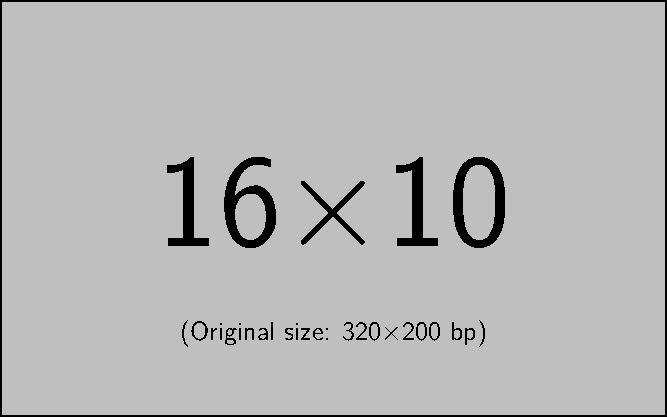
\includegraphics[width=0.75\linewidth]{example-image-16x10.pdf}
% % % \caption{Insert figure caption here}
% % % \label{fig_sim}
% % % \end{figure}


% % % \begin{figure*}
% % % \centering
% % % 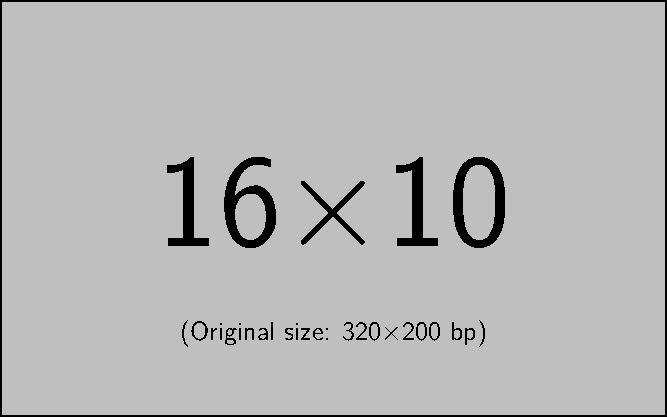
\includegraphics[width=0.8\linewidth]{example-image-16x10.pdf}
% % % \caption{Insert figure caption here}
% % % \label{fig_wide}
% % % \end{figure*}


% % % See example table in Table~\ref{table_example}.

% % % \begin{table}[hbt!]
% % % \begin{threeparttable}
% % % \caption{An Example of a Table}
% % % \label{table_example}
% % % \begin{tabular}{llll}
% % % \toprule
% % % \headrow Column head 1 & Column head 2  & Column head 3 & Column head 4\\
% % % \midrule
% % % One\tnote{a} & Two&three three &four\\ 
% % % \midrule
% % % Three & Four&three three\tnote{b} &four\\
% % % \bottomrule
% % % \end{tabular}
% % % \begin{tablenotes}[hang]
% % % \item[]Table note
% % % \item[a]First note
% % % \item[b]Another table note
% % % \end{tablenotes}
% % % \end{threeparttable}
% % % \end{table}


% % % \section{Conclusion}
% % % The conclusion text goes here.


% % % \paragraph{Acknowledgments}
% % % We are grateful for the technical assistance of A. Author.


% % % \paragraph{Funding Statement}
% % % This research was supported by grants from the <funder-name><doi>(<award ID>); <funder-name><doi>(<award ID>).

% % % \paragraph{Competing Interests}
% % % A statement about any financial, professional, contractual or personal relationships or situations that could be perceived to impact the presentation of the work --- or `None' if none exist

% % % \paragraph{Data Availability Statement}
% % % A statement about how to access data, code and other materials allowing users to understand, verify and replicate findings --- e.g. Replication data and code can be found in Harvard Dataverse: \verb+\url{https://doi.org/link}+.

% % % \paragraph{Ethical Standards}
% % % The research meets all ethical guidelines, including adherence to the legal requirements of the study country.

% % % \paragraph{Author Contributions}
% % % Please provide an author contributions statement using the CRediT taxonomy roles as a guide {\verb+\url{https://www.casrai.org/credit.html}+}. Conceptualization: A.A; A.B. Methodology: A.A; A.B. Data curation: A.C. Data visualisation: A.C. Writing original draft: A.A; A.B. All authors approved the final submitted draft.


% % %\endnote in some journals will behave like \footnote; and \printendnotes will not output anything. 
% % % \printendnotes

% % % \defbibnote{preamble}{By default, this template uses \texttt{biblatex} and adopts the Chicago referencing style. However, the journal you’re submitting to may require a different reference style; specify the journal you're using with the class' \texttt{journal} option --- see lines 1--13 of \emph{sample.tex} for a list of options and instructions for selecting the journal.}

\printbibliography
% % % \appendix

% % % \section{Example Appendix Section}

% % % Lorem ipsum dolor sit amet, consectetur adipiscing elit, sed do eiusmod tempor incididunt ut labore et dolore magna aliqua. Lorem ipsum dolor sit amet, consectetur adipiscing elit, sed do eiusmod tempor incididunt ut labore et dolore magna aliqua. Lorem ipsum dolor sit amet, consectetur adipiscing elit, sed do eiusmod tempor incididunt ut labore et dolore magna aliqua. 

\end{document}